\chapter{Implementación}

Como ya se explicó en el Capítulo \ref{ch:planificación} la implementación del proyecto se ha llevado a cabo en una serie de \textbf{Sprints}. Estos se han definido en \textbf{GitHub} a modo de \textit{hitos} y cada uno de ellos contendrá un grupo de \textit{issues} que corresponden a las diferentes \textbf{Historias de Usuario} y \textbf{Tareas} que se han ido incorporando al proyecto a lo largo desarrollo del mismo. \\

\section{Creación del Bot}

La creación de un Bot de \textbf{Telgram} es un proceso muy simple, ya que podemos hacerlos desde la propia aplicación. \textbf{Telegram} tiene su propio Bot implementado que permite crear el resto de estos, este es \textbf{@BotFather}. Al iniciar la comunicación con este Bot lo primero que se nos dará será un listado de las diferentes opciones de las que disponemos para crear, editar, eliminar un Bot entre otras, como puede verse en la Figura \ref{fig:crear-bot-1}.

\begin{figure}[p]
	\centering
	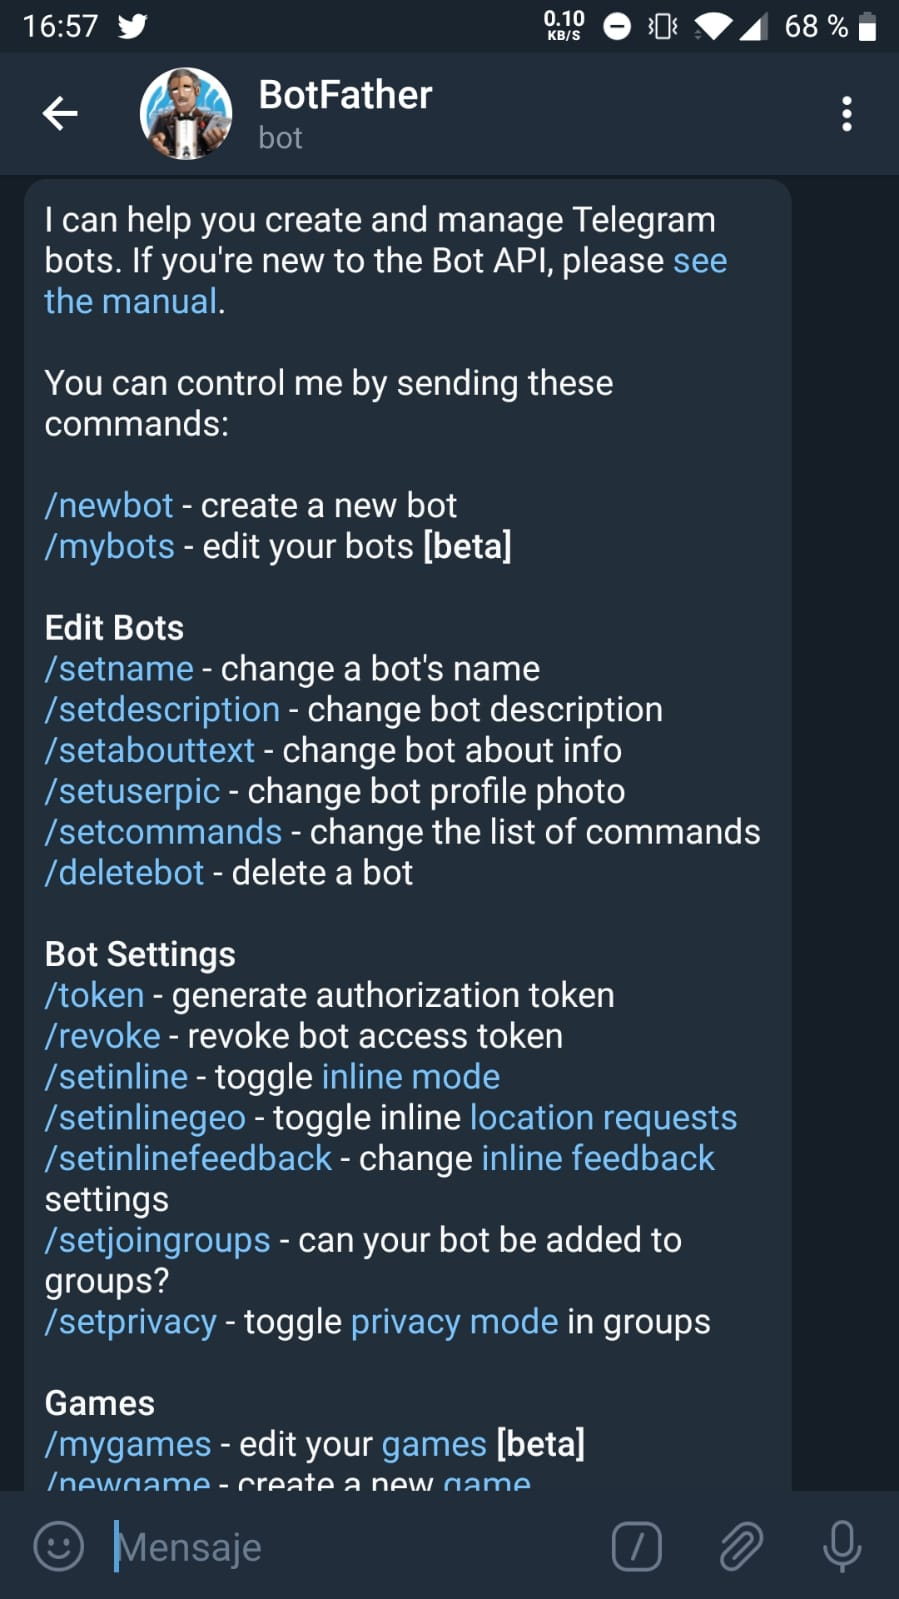
\includegraphics[width=0.8\textwidth]{img/crear-bot-1}
	\caption{Opciones disponibles de @BotFather.}
	\label{fig:crear-bot-1}
\end{figure}

Para crear el Bot tendremos que seleccionar (o escribir) el comando \textbf{/newbot} y el propio \textbf{BotFather} nos pedirá el nombre que queremos darle junto con el nombre de usuario que tendrá en \textbf{Telegram} (terminando este siempre en "bot"). Tras introducirlos, \textbf{BotFather} nos proveerá del TOKEN necesario para poder acceder a la API de \textbf{Telegram} con nuestro Bot, como puede verse en la Figura \ref{fig:crear-bot-2}

\begin{figure}[p]
	\centering
	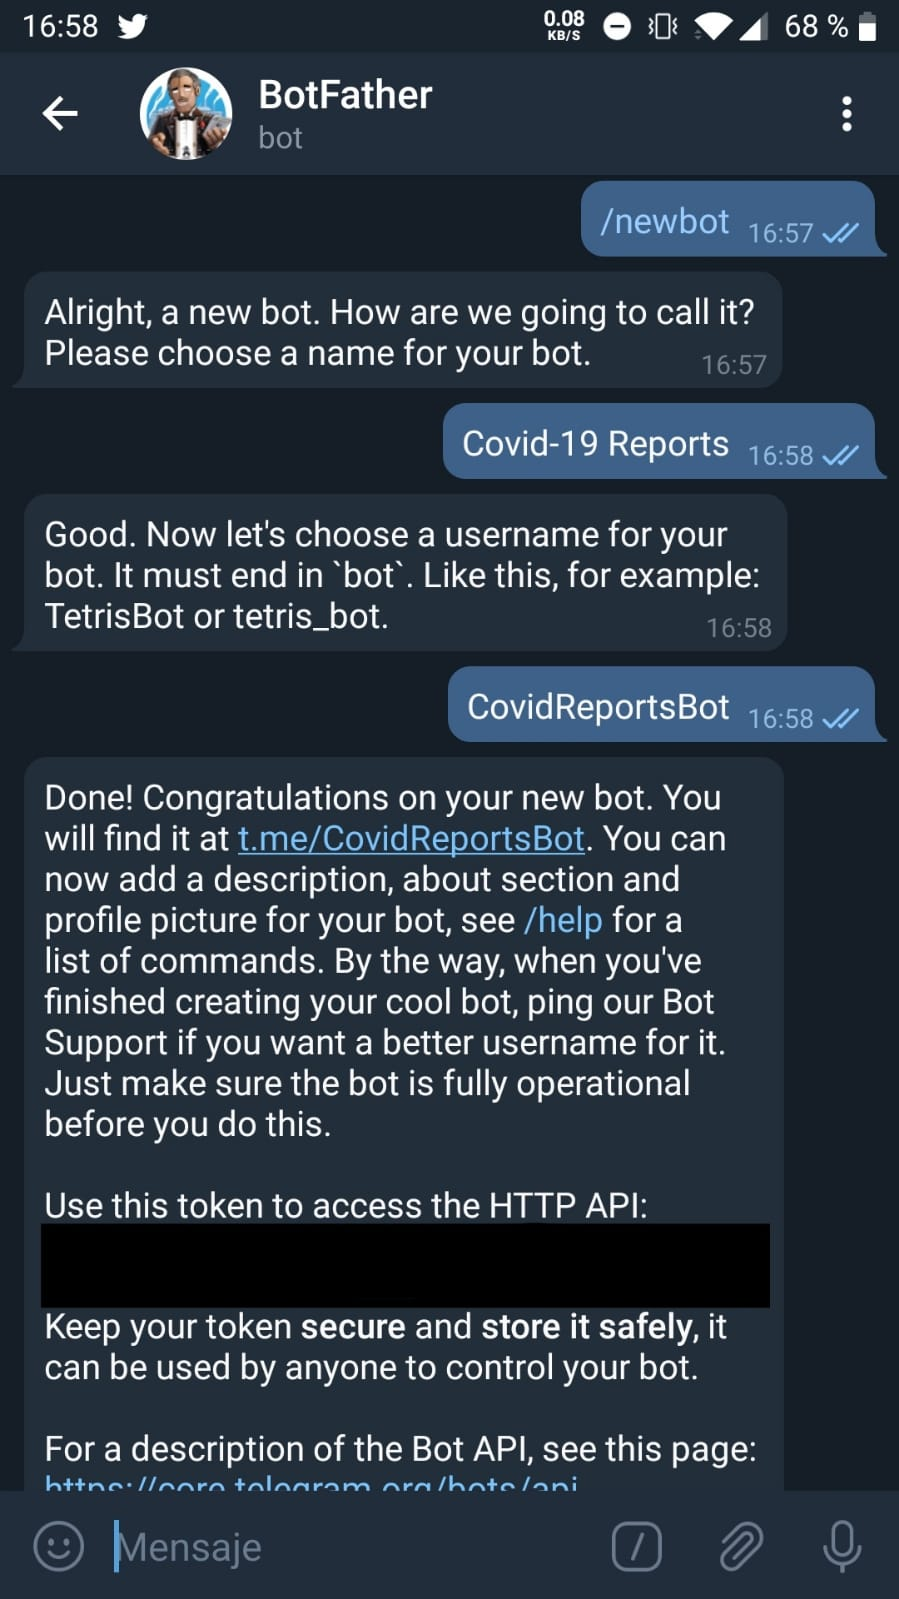
\includegraphics[width=0.8\textwidth]{img/crear-bot-2}
	\caption{Creación del Bot.}
	\label{fig:crear-bot-2}
\end{figure}

Como ya se mencionó en la Sección \ref{sec:recursos}, usaremos la biblioteca \textbf{python-telegram-bot} para implementar el Bot, así como \textbf{Heroku} para llevar a clavo su despliegue. Como base para desarrollar el Bot se tomó el artículo de Artem Rys \cite{crear-bot-heroku} donde se nos explica como crear un Bot haciendo uso de esta biblioteca y como configurar \textbf{Heroku} para su despliegue en la plataforma.

\section{Implementación del Bot}

A lo largo de este apartado se explicarán como se ha llevado a cabo la implementación del Bot mostrando código del mismo.

\subsection{Handlers}

Para poder majenar las diferentes acciones que realizará el Bot se ha hecho uso de una serie de \textbf{handlers} que nos proporciona la propia biblioteca \textbf{python-telegram-bot}. En este caso, entre los diferentes \textbf{handlers} que puede proveernos esta biblioteca a lo largo del proyecto se han utilizado los siguientes:

\begin{itemize}
	\item \textbf{CallbackQueryHandler:} con la siguiente estructura en su llamada \textit{CallbackQueryHandler(callback, pattern), este handler se encargará de ejecutar la función definida en el \textit{callback} cuando se pulse un botón cuyo \textit{pattern} coincide con el del handler.
	\item \textbf{CommandHandler:} con la siguiente estructura en su llamada \textit{CommandHandler(command, callback)}, este handler se encargará de de ejecutar la función definida en el \textit{callback} cuando reciba el \textit{command} (comando)) correcto (los comandos de \textbf{Telegram} son aquellos mensajes que comienzan por \textbf{/}).
	\item \textbf{MessageHandler:} con la siguiente estructura en su llamada \textit{MessageHandler(filters, callback)}, este handler se encargará de de ejecutar la función definida en el \textit{callback} cuando reciba reciba un mensaje que cumpla con las condiciones definidas en su \textit{filters} (filtros)}.
\end{itemize}

\subsection{Funciones de respuesta}

Como hemos dicho con anterioridad, este Bot será de tipo conversacional. Esto conlleva que el Bot tendrá que responder a las solicitudes que el usuario le realice. Para ello se han definido una serie de funciones que, haciendo uso de los \textbf{handlers} definidos en el apartado anterior compondrán nuestro Bot, permitiendo reponder al usuario.

Estas funciones estarán caracterizadas por estar definidas todas con dos parámetros (\textbf{update} y \textbf{context}) los cuales contienen información del mensaje enviado (nombre y apellidos del usuario, alias, identificador del chat). Podemos verlo en el Listing \ref{lst:def-funcion}

\lstset{
	backgroundcolor=\color{white},
	basicstyle=\footnotesize,
	breakatwhitespace=false,         
	breaklines=true,
	captionpos=b,
	commentstyle=\color{green},
	extendedchars=true,              
	frame=single,
	keepspaces=true,
	keywordstyle=\color{blue},
	language=Python,
	numbers=left,
	numbersep=5pt,
	numberstyle=\small\color{black},
	showstringspaces=false,
	rulecolor=\color{black},
	stringstyle=\color{blue},
	tabsize=2,
	texcl=true
}

\begin{lstlisting}[language=Python, caption={Definición de un función usada por los handler.}, label={lst:def-funcion}]
def nombre_funcion ( update , context ) :
\end{lstlisting}

Para facilitar el entendimiento, mostraremos los diferentes modelos de funciones que se han utilizado para implementar el Bot, evitando así exponer todo el código del mismo ya que la estructura de las funciones es la misma dependiendo del tipo. Dentro de los diferentes tipos de funciones implementada, las dividiremos según el tipo de respuestas que estas nos ofrecen.

\subsubsection{Función para iniciar el Bot}

La primera función que definirá el Bot será su funcionó de inicio, la cual permitirá poder empezar a utilizar el Bot y creará los botones de los menús en el teclado del usuario. Desglosaremos el código del Listing \ref{lst:def-funcion-inicio}:

\begin{itemize}
	\item \textbf{Lineas 1 y 2:} Recogen en dos variables los valores del nombre del usuario y el identificador del chat desde los parámetros.
	\item \textbf{Lineas 4 a 7:} Comprueba que el usuriario tiene un usuario de \textbf{Telegram} y si no lo tiene le informa de como hacerlo.
	\item \textbf{Lineas 11 a 13:} Se crea una lista con los botones del teclado que se quieren mostrar al usuario. A diferencia de los botones que se muestran en el chat, estos carecen de un parámetro \textbf{callback\_data}.
	\item \textbf{Lineas 15 a 17:} Se crea el objeto que contendrá los botones y se le especifica que quiere que se adapte al tamaño del teclado (\textbf{resize\_keyboard}), así como que quiere que siempre se mantenga visible (\textbf{one\_time\_keyboard}).
	\item \textbf{Lineas 19 a 22:} Se usará la función \textbf{reply\_text} sobre el mensaje que nos da el Bot para añadirle el texto que queremos que este devuelva, asi como un parámetro adicional (\textbf{reply\_markup}) donde se encuentra el listado de botones del menú del teclado.
\end{itemize}

\begin{lstlisting}[language=Python, caption={Función de inicio del Bot.}, label={lst:def-funcion-inicio}]
chat_id = update.effective_user["id"]
username = update.message.chat.username

if username is None:
	logger.info("User {} started bot".format('None:' + str(chat_id)))
	update.message.reply_text("Bienvenido a Covid-19 Report! Parece que no tienes usuario de Telegram."
							  " Ve a ajustes, ponte un nombre de usuario y podremos empezar.")
else:
	logger.info("User {} started bot".format(username + ':' + str(chat_id)))

	main_menu_keyboard = [[KeyboardButton("Menu"),
						   KeyboardButton("Ayuda"),
						   KeyboardButton("Informacion")]]

	reply_kb_markup = ReplyKeyboardMarkup(main_menu_keyboard,
										  resize_keyboard=True,
										  one_time_keyboard=False)

update.message.reply_text(text="Bienvenido a Covid-19 Report! {}\n"
							   "Gracias a este bot podras conocer el estado de la situacion actual provocada "
							   "por el Covid-19.".format(username),
						  reply_markup=reply_kb_markup)
\end{lstlisting}

\subsubsection{Función responde con texto}

En este apartado analizaremos como que implementa una función para cuando el Bot solo devuelva texto. Desglosaremos el código del Listing \ref{lst:def-funcion-texto}:

\begin{itemize}
	\item \textbf{Lineas 1:} Se usará la función \textbf{reply\_text} para añadirle el texto que se quiere que el Bot devuelva cuando el \textbf{handler} llame a la función.
\end{itemize}

\begin{lstlisting}[language=Python, caption={Función que devuelve texto en el chat.}, label={lst:def-funcion-texto}]
update.message.reply_text("Usa /start para iniciar el bot")
\end{lstlisting}

\subsubsection{Función responde con texto y botones}

En este apartado analizaremos como que implementa una función para cuando el Bot devuelva texto y botones. Desglosaremos el código del Listing \ref{lst:def-funcion-texto-botones}:

\begin{itemize}
	\item \textbf{Lineas 1 a 6:} Se creará una lista con los botones que el Bot mostrará al usuario. Estos contendrán un parámetro \textbf{callback\_data} donde se definirá el nombre del callback para que al pulsar el botón el \textbf{handler CallbackQueryHandler} ejecute la función asociada a este callback.
	\item \textbf{Lineas 8 a 11:} Se usará la función \textbf{reply\_text} para añadirle el texto que se quiere que el Bot devuelva cuando el \textbf{handler} llame a la función, asi como un parámetro adicional (\textbf{reply\_markup}) donde se encuentra el listado de botones que mostrará el Bot en el chat.
\end{itemize}

\begin{lstlisting}[language=Python, caption={Función que devuelve texto y botones en el chat.}, label={lst:def-funcion-texto-botones}]
keyboard = [
	[InlineKeyboardButton("Andalucia", callback_data='andalucia_info'),
	InlineKeyboardButton("Aragon", callback_data='aragon_info'),
	InlineKeyboardButton("Asturias", callback_data='asturias_info')],
	]
reply_markup = InlineKeyboardMarkup(keyboard)

message.reply_text(
	text="{} elige la comunidad de la que quieres consultar datos.".format(username),
	reply_markup=reply_markup
)
\end{lstlisting}

\subsubsection{Función responde con imagen}

En este apartado analizaremos como que implementa una función para cuando el Bot solo devuelva texto. Desglosaremos el código del Listing \ref{lst:def-funcion-imagen}:

\begin{itemize}
	\item \textbf{Lineas 1:} Se usará la función \textbf{reply\_text} hacer que el Bot envía la imagen al chat cuando el \textbf{handler} llame a la función que contiene el código.
	\item \textbf{Lineas 2:} Se usará la función \textbf{open} para abrir la imagen que se encuentra en la \textbf{ruta}, indicando el parámetro \textbf{rb} que se abrirá con representación binaria
\end{itemize}

\begin{lstlisting}[language=Python, caption={Función que devuelve una imagen en el chat.}, label={lst:def-funcion-imagen}]
message.reply_photo(
	photo=open('ruta', 'rb')
)
\end{lstlisting}

\subsection{Fallbacks}

Al tratarse de un Bot conversacional, una de las cosas principales que se ha de tener en cuenta en el momento de su implementación es que este no puede dar información que no corresponda con el contexto en el que se encuentra. Un ejemplo en \textbf{Covid-19 Reports} sería estando en el contexto de consulta de los datos una provincia, preguntarle por la información de los casos de España.

Ahora pasaremos a mostrar como funcionan los \textbf{fallbacks}. En primer lugar, se han definido una serie de \textbf{contextos} sobre los que el Bot puede actuar. Un ejemplo de estos seria el contexto \textbf{INICIO}, donde definiremos los diferentes \textbf{handler} con las respuestas posibles que el Bot podría darnos en este contexto como se muestra en el Listing \ref{lst:contexto}

\begin{lstlisting}[language=Python, caption={Lista de handlers asociado al conexto INICIO.}, label={lst:contexto}]
INICIO: [
	MessageHandler(Filters.regex('Menu'), show_inicio),
	MessageHandler(Filters.regex('Ayuda'), help_handler),
	MessageHandler(Filters.regex('Informacion'), show_info),
	MessageHandler(Filters.text & (~Filters.command), any_message),
	CallbackQueryHandler(show_andalucia_info, pattern='andalucia_info'),
	CallbackQueryHandler(show_aragon_info, pattern='aragon_info'),
	CallbackQueryHandler(show_asturias_info, pattern='asturias_info'),
	CallbackQueryHandler(show_cvalenciana_info, pattern='cvalenciana_info'),
	CallbackQueryHandler(show_canarias_info, pattern='canarias_info'),
	CallbackQueryHandler(show_cantabria_info, pattern='cantabria_info'),
	CallbackQueryHandler(show_castillalamancha_info, pattern='castillalamancha_info'),
	CallbackQueryHandler(show_castillayleon_info, pattern='castillayleon_info'),
	CallbackQueryHandler(show_cataluna_info, pattern='cataluna_info'),
	CallbackQueryHandler(show_ceuta_info, pattern='ceuta_info'),
	CallbackQueryHandler(show_extremadura_info, pattern='extremadura_info'),
	CallbackQueryHandler(show_galicia_info, pattern='galicia_info'),
	CallbackQueryHandler(show_baleares_info, pattern='baleares_info'),
	CallbackQueryHandler(show_larioja_info, pattern='larioja_info'),
	CallbackQueryHandler(show_madrid_info, pattern='madrid_info'),
	CallbackQueryHandler(show_melilla_info, pattern='melilla_info'),
	CallbackQueryHandler(show_murcia_info, pattern='murcia_info'),
	CallbackQueryHandler(show_navarra_info, pattern='navarra_info'),
	CallbackQueryHandler(show_paisvasco_info, pattern='paisvasco_info'),
	CallbackQueryHandler(show_espana_info, pattern='espana_info'),
],
\end{lstlisting}

Como se puede ver, en este contexto el Bot presenta una diversidad de opciones asociadas tanto a botones como con texto que se puede introducir. Pero, ¿que pasa si se produce un acción en otro contexto? Para ello existen los \textbf{fallbacks}. Los \textbf{fallbacks} estarán representados en una lista donde se implementarán los \textbf{handlers} que no se encuentran en el contexto correcto. Por ello, como podremos ver en el Listing \ref{lst:fallback}, se han definido los mismos \textbf{handlers} implementados en el Listing \ref{lst:contexto}. Esto es porque estos mismos handlers pueden no corresponder a cualquier otro contexto, por lo que el \textbf{fallback} asociado al \textbf{pattern} se encargará de llamar a otra función diferente a la original de manera que se realice una acción diferente. Para \textbf{Covid-19 Reports}, esa opción será la de mostrar un mensaje comunicando que no se encuentra en el contexto de la petición.

\begin{lstlisting}[language=Python, caption={Fallbacks.}, label={lst:fallback}]
INICIO: [
	CommandHandler('start', start_handler),
	CommandHandler('help', help_handler),
	CommandHandler('info', show_info),
	CallbackQueryHandler(usuario_pulsa_boton_anterior,
	pattern='start_menu'),
	CallbackQueryHandler(usuario_pulsa_boton_anterior, pattern='andalucia_info'),
	CallbackQueryHandler(usuario_pulsa_boton_anterior, pattern='aragon_info'),
	CallbackQueryHandler(usuario_pulsa_boton_anterior, pattern='asturias_info'),
	CallbackQueryHandler(usuario_pulsa_boton_anterior, pattern='cvalenciana_info'),
	CallbackQueryHandler(usuario_pulsa_boton_anterior, pattern='canarias_info'),
	CallbackQueryHandler(usuario_pulsa_boton_anterior, pattern='cantabria_info'),
	CallbackQueryHandler(usuario_pulsa_boton_anterior, pattern='castillalamancha_info'),
	CallbackQueryHandler(usuario_pulsa_boton_anterior, pattern='castillayleon_info'),
	CallbackQueryHandler(usuario_pulsa_boton_anterior, pattern='cataluna_info'),
	CallbackQueryHandler(usuario_pulsa_boton_anterior, pattern='ceuta_info'),
	CallbackQueryHandler(usuario_pulsa_boton_anterior, pattern='extremadura_info'),
	CallbackQueryHandler(usuario_pulsa_boton_anterior, pattern='galicia_info'),
	CallbackQueryHandler(usuario_pulsa_boton_anterior, pattern='baleares_info'),
	CallbackQueryHandler(usuario_pulsa_boton_anterior, pattern='larioja_info'),
	CallbackQueryHandler(usuario_pulsa_boton_anterior, pattern='madrid_info'),
	CallbackQueryHandler(usuario_pulsa_boton_anterior, pattern='melilla_info'),
	CallbackQueryHandler(usuario_pulsa_boton_anterior, pattern='murcia_info'),
	CallbackQueryHandler(usuario_pulsa_boton_anterior, pattern='navarra_info'),
	CallbackQueryHandler(usuario_pulsa_boton_anterior, pattern='paisvasco_info'),
	CallbackQueryHandler(usuario_pulsa_boton_anterior, pattern='espana_info'),
],
\end{lstlisting}

Como puede verse, también se han usado algunos \textbf{CommandHandler}, dado que queremos permitir que en cualquier contexto estos puedan llamar a sus respectivas funciones.

\subsection{Funciones análisis de datos}

Para poder llevar a cabo la implementación del análisis de datos, en primer lugar, debemos saber como están estos datos estructurados. Los datos que se van a utilizar para implementar el Bot los conseguiremos desde el \textbf{GitHub de Datadista} \cite{github-datadista}. Al tratarse de archivos tipo \textit{.csv} se optó por hacer uso de la librería \textbf{pandas} como se dijo en la Sección \ref{sec:recursos}.

Para poder cargar la información de estos archivos se usará la función de \textbf{pandas} \textbf{read\_csv}, pudiendo ver un ejemplo en el Listing \ref{lst:read-csv}. De los parámetros que se utilizan en esta función, \textbf{usecols} es el único que no se usa en todos los casos, dado que éste sirve para indicar, mediante una lista, las columnas que se querrán cargar en el \textbf{dataframe}. Los otros dos parámetros nos indicarán, en primer lugar conde se puede encontrar el archivo, ya sea en una ruta definida en algún directorio como una url que contenga los datos, y el parámetro \textbf{sep} indicará cual es el caracter separador a tener en cuenta.

\begin{lstlisting}[language=Python, caption={Función read\_csv.}, label={lst:read-csv}]
df = pd.read_csv('ruta/url', sep=',', usecols=list_columns)
\end{lstlisting}

Una vez cargados los datos en sus correspondientes \textbf{dataframes} se procede a trabajar con ellos para obtener los datos que queremos que el Bot devuelva al usuario.

Para un mayor claridad, explicaremos la estructura de los diferentes \textbf{dataframes} y lo que representa cada uno de sus valores.

\subsubsection{Dataframe casos por Comunidad Autónoma}

Este \textbf{dataframe} contendrá la información del nº de casos que se han producido en cada Comunidad Autónoma en una fecha concreta. Éste tendrá la siguiente estructura:

\begin{center}
	\textit{(fecha, ccaa, num\_casos)}
\end{center}

\begin{itemize}
	\item \textbf{fecha:} clave principal, fecha en formato YYYY-mm-dd.
	\item \textbf{ccaa:} nombre de la Comunidad Autónoma.
	\item \textbf{num\_casos:} nº de casos detectados en la Comunidad Autónoma en la fecha.
\end{itemize}

\subsubsection{Dataframe fallecidos por Comunidad Autónoma}

Este \textbf{dataframe} contendrá la información del nº de fallecimientos que se han producido en cada Comunidad Autónoma en una fecha concreta. Éste tendrá la siguiente estructura:

\begin{center}
	\textit{(Fecha, CCAA, Fallecidos)}
\end{center}

\begin{itemize}
	\item \textbf{Fecha:} clave principal, fecha en formato YYYY-mm-dd.
	\item \textbf{CCAA:} nombre de la Comunidad Autónoma.
	\item \textbf{Fallecidos:} nº de fallecidos confirmados en la Comunidad Autónoma en la fecha.
\end{itemize}

\subsubsection{Dataframe datos hospitalización por Comunidad Autónoma}

Este \textbf{dataframe} contendrá la información de los datos hospitalarios que se han producido en cada Comunidad Autónoma y en España en una fecha concreta. Éste tendrá la siguiente estructura:

\begin{center}
	\textit{(Fecha, CCAA, Total Pacientes COVID ingresados, \% Camas Ocupadas COVID, Total pacientes COVID en UCI, \% Camas Ocupadas UCI COVID, Ingresos COVID últimas 24 h, Altas COVID últimas 24 h)}
\end{center}

\begin{itemize}
	\item \textbf{Fecha:} clave principal, fecha en formato YYYY-mm-dd.
	\item \textbf{CCAA:} nombre de la Comunidad Autónoma (o España).
	\item \textbf{Total Pacientes COVID ingresados:} nº de pacientes Covid que se encuentran hospitalizados en la fecha.
	\item \textbf{\% Camas Ocupadas COVID:} \% de las camas disponibles en hospitales ocupada por pacientes Covid en la fecha.
	\item \textbf{Total pacientes COVID en UCI:} nº de pacientes Covid que se encuentran hospitalizados en UCI en la fecha.
	\item \textbf{\% Camas Ocupadas UCI COVID:} \% de las camas UCI disponibles en hospitales ocupada por pacientes Covid en la fecha.
	\item \textbf{Ingresos COVID últimas 24 h:} nº de pacientes ingresados en las últimas 24 horas en la fecha.
	\item \textbf{Altas COVID últimas 24 h:} nº de pacientes dados de alta en las últimas 24 horas en la fecha.
\end{itemize}

\subsubsection{Dataframe casos y fallecimiento por rango de edad}

Este \textbf{dataframe} contendrá la información del nº de casos y fallecidos que se han producido en el país por rango de edad y sexo en una fecha concreta. Éste tendrá la siguiente estructura:

\begin{center}
	\textit{(fecha, rango\_edad, sexo, casos\_confirmados, hospitalizados, ingresos\_uci, fallecidos)}
\end{center}

\begin{itemize}
	\item \textbf{fecha:} clave principal, fecha en formato YYYY-mm-dd.
	\item \textbf{rango\_edad:} rango de edad donde se han producido los casos, divididos en intervalos de 10 años, desde \textit{0-9} hasta \textit{80 y +}. También existe un \textit{Total} de los datos.
	\item \textbf{sexo:} indicará el sexo de la población, dividiendose en \textit{hombres}, \textit{mujeres} y \textit{ambos}.
	\item \textbf{casos\_confirmados:} nº de casos detectados por edad y rango en la fecha.
	\item \textbf{hospitalizados:} nº de pacientes Covid hospitalizados por edad y rango en la fecha.
	\item \textbf{ingresos\_uci:} nº de pacientes Covid hospitalizados en UCI por edad y rango en la fecha.
	\item \textbf{fallecidos:} nº de fallecidos confirmados por edad y rango en la fecha.
\end{itemize}

\subsubsection{Dataframe nº de habitantes por Comunidad Autónoma}

Este \textbf{dataframe} contendrá la información del nº de habitantes de cada Comunidad Autónoma. Éste tendrá la siguiente estructura:

\begin{center}
	\textit{(ccaa, habitantes)}
\end{center}

\begin{itemize}
	\item \textbf{ccaa:} clave principal, nombre de cada Comunidad Autónoma de España.
	\item \textbf{habitantes:} nº total de habitantes de cada Comunidad Autónoma.
\end{itemize}

Para evitar repetir el código, se mostrará las funciones que se usan sobre estos \textbf{dataframes} a lo largo del proyecto presentándolos en los Listing \ref{lst:funcion-1} a \ref{lst:funcion-2}.

En el Listing \ref{lst:funcion-1} se muestra el uso de dos funciones, \textbf{groupby} y \textbf{sum}, las cuales en el ejemplo, se usan para poder devolver la sumatoria de los casos agrupados por Comunidades, seleccionando por último la Comunidad de la que se quiere conocer la sumatoria de sus casos.

\begin{itemize}
	\item \textbf{Función groupby:} Esta será la encargada de agrupar los datos según la columna elegida, la cual no identifica a la clave del dataframe, en este caso la columna \textit{ccaa}. 
	\item \textbf{Función sum:} Ésta será la encargada de realizar la sumatoria de los valores seleccionados. Es este ejemplo, tras agrupar los datos por Comunidades, se realizará la sumatoria del nº de casos de las mismas.
\end{itemize}

\begin{lstlisting}[language=Python, caption={Funciones groupby y sum.}, label={lst:funcion-1}]
df_ccaa_casos.groupby(['ccaa'])['num_casos'].sum()[current_autonomy]
\end{lstlisting}

En el Listing \ref{lst:funcion-2} se muestra el uso de la función \textbf{loc}. Ésta se usa a lo largo del proyecto para crear nuevos dataframes que cumplan una serie de condiciones simultaneas, por ejemplo, seleccionar los datos de una Comunidad concreta en una fecha deseada.

\begin{itemize}
	\item \textbf{Función loc:} Esta será la encargada de, por medio de las condiciones definidad en si interior, crear un nuevo dataframe que cumpla las mismas.
	\item \textbf{Values:} Values se usará para obtener el valor de una columna, es este caso, el primer valor de la comuna \textit{col}.
\end{itemize}

\begin{lstlisting}[language=Python, caption={Función loc.}, label={lst:funcion-2}]
df_loc = df.loc[(condicion_1) & (condicion_2)]

df_loc['col'].values[0]
\end{lstlisting}

Por medio de estas funciones se hará una selección de los datos que el Bot ha demostrar al usuario, pudiendo combinarlas entre ellas para obtener diferentes datos.

\subsection{Funciones de creación de gráficas}

Para permitir que el Bot pueda crear diferentes imágenes que muestren gráficos y las muestre junto a los datos que se obtienen en el punto anterior se ha hecho uso de la biblioteca \textbf{matplotlib}. Esta nos permitirá crear gráficos haciendo uso de los datos de los \textbf{dataframes}.

Existen diferentes tipos de gráficos que se pueden usar. Para este proyecto dependiendo del los tipos de datos se han elegido diferentes modelos de gráficos: barras, barras laterales, tramas.

\subsubsection{Gráficos de barras y tramas}

Para los gráficos de barras y tramas se ha seguido la estructura que de muestra en el Listing \ref{lst:barras}. 

\begin{itemize}
	\item \textbf{Lineas 1 y 2:} Se creará creará un nuevo \textbf{dataframe} con los datos de los que se desea mostrar y por medio de la función \textbf{set\_index} se asignará la columna del \textbf{dataframe} como el index del mismo.
	\item \textbf{Lineas 4:} Se creará el tamaño de la imágen y se crearán las variables \textbf{fig} y \textbf{ax} que se usarán mas adelante.
	\item \textbf{Lineas 5:} Se creará una variable que contendrá un objeto \textit{Index} que será el que contenga los indices de la gráfica.
	\item \textbf{Lineas 7:} Se creará la gráfica de barras, donde los parámetros introducisos serán el Index creado antes, el listado de valores correspondientes a cada index, así como la opacidad de la barra (alpha) y el grosor de éstas (width).
	\item \textbf{Lineas 8:} Se creará la gráfica de tramas, donde los parámetros introducisos serán el Index creado antes, el listado de valores correspondientes a cada index, así como el color de la misma.
	\item \textbf{Lineas 10:} Se indicarán los valores que se representarán en el axis de la gráfica.
	\item \textbf{Lineas 11:} Se indicarán los valores de inicio y final que se representarán en el axis de la gráfica.
	\item \textbf{Lineas 12:} Se formateará como se muestras los diferentes valores de axis.
	\item \textbf{Lineas 14 y 15:} Se le da nombre a la gráfica así como a su eje y.
	\item \textbf{Lineas 16 y 17:} Crea el archivo con la gráfica en el directorio seleccionado y posteriormente cerraremos la figura para evitar problemas al crear otras gráficas.
\end{itemize}

\begin{lstlisting}[language=Python, caption={Generár gráficos de barras y tramas.}, label={lst:barras}]
df_casos_fecha = df_ccaa_casos.groupby('fecha')['num_casos'].sum().reset_index()
df_casos_fecha.set_index("fecha", inplace=True)

fig, ax = plt.subplots(figsize=(12, 6))
x = df_casos_fecha.index.get_level_values('fecha')

plt.bar(x, df_casos_fecha['num_casos'], alpha=0.5, width=0.5)
plt.plot(x, df_casos_fecha['num_casos'], color='red')

ax.set_xticks(inicio_mes)
ax.set_xlim('2020-03-01', x[-1])
ax.figure.autofmt_xdate()

plt.title('Incremento de casos en Espana', fontsize=26)
ax.set_ylabel('N Casos', fontsize=15)
plt.savefig('./img_graficas/incremento_espana.png')
plt.close()
\end{lstlisting}

\subsubsection{Gráficos de barras laterales}

Para los gráficos de barras y tramas se ha seguido la estructura que de muestra en el Listing \ref{lst:barras-laterales}. 

\begin{itemize}
	\item \textbf{Lineas 1 y 2:} Se creará creará un nuevo \textbf{dataframe} con los datos de los que se desea mostrar y por medio de la función \textbf{set\_index} se asignará la columna del \textbf{dataframe} como el index del mismo.
	\item \textbf{Lineas 4:} Se creará el tamaño de la imágen y se crearán las variables \textbf{fig} y \textbf{ax} que se usarán mas adelante.
	\item \textbf{Lineas 5:} Se creará una variable que contendrá un objeto \textit{Index} que será el que contenga los indices de la gráfica.
	\item \textbf{Lineas 7:} Se creará la gráfica de barra laterales, donde los parámetros introducisos serán el Index creado antes, el listado de valores correspondientes a cada index, así como la opacidad de la barra (alpha) y el grosor de éstas (width).
	\item \textbf{Lineas 9:} Se formateará como se muestras los diferentes valores de axis.
	\item \textbf{Lineas 11 y 12:} Se le da nombre a la gráfica y se invertirá si eje y.
	\item \textbf{Lineas 14 y 15:} Se le añadirá al final de cada barra el valor que representa la misma.
	\item \textbf{Lineas 17 y 18:} Crea el archivo con la gráfica en el directorio seleccionado y posteriormente cerraremos la figura para evitar problemas al crear otras gráficas.
\end{itemize}

\begin{lstlisting}[language=Python, caption={Generár gráficos de barras laterales.}, label={lst:barras-laterales}]
df_casos_fecha = df_ccaa_casos.groupby('fecha')['num_casos'].sum().reset_index()
df_casos_fecha.set_index("fecha", inplace=True)

fig, ax = plt.subplots(figsize=(12, 6))
x = df_casos_fecha.index.get_level_values('fecha')

plt.barh(x, df['n_casos'], alpha=0.5, height=0.8)

ax.figure.autofmt_xdate()

plt.title('Incremento de casos en Espana', fontsize=26)
plt.gca().invert_yaxis()

for index, value in enumerate(df['n_casos']):
plt.text(value, index, str(value))

plt.savefig('./img_graficas/incremento_espana.png')
plt.close()
\end{lstlisting}

